\documentclass{article}
\usepackage[utf8x]{inputenc}
\usepackage{ucs}
\usepackage{amsmath} 
\usepackage{amsfonts}
\usepackage{upgreek}
\usepackage[english,russian]{babel}
\usepackage{graphicx}
\usepackage{float}
\usepackage{textcomp}
\usepackage{hyperref}
\usepackage{geometry}
  \geometry{left=2cm}
  \geometry{right=1.5cm}
  \geometry{top=1cm}
  \geometry{bottom=2cm}
\usepackage{tikz}
\usepackage{ccaption}
\usepackage{multicol}

\usepackage{listings}
%\setlength{\columnsep}{1.5cm}
%\setlength{\columnseprule}{0.2pt}


\begin{document}
\pagenumbering{gobble}

\lstset{
  language=C,                % choose the language of the code
  basicstyle=\linespread{1.1}\ttfamily,
  columns=fixed,
  fontadjust=true,
  basewidth=0.5em,
  keywordstyle=\color{blue}\bfseries,
  commentstyle=\color{gray},
  stringstyle=\ttfamily\color{orange!50!black},
  showstringspaces=false,
  %numbers=false,                   % where to put the line-numbers
  numbersep=5pt,
  numberstyle=\tiny\color{black},
  numberfirstline=true,
  stepnumber=1,                   % the step between two line-numbers.        
  numbersep=10pt,                  % how far the line-numbers are from the code
  backgroundcolor=\color{white},  % choose the background color. You must add \usepackage{color}
  showstringspaces=false,         % underline spaces within strings
  captionpos=b,                   % sets the caption-position to bottom
  breaklines=true,                % sets automatic line breaking
  breakatwhitespace=true,         % sets if automatic breaks should only happen at whitespace
  xleftmargin=.2in,
  extendedchars=\true,
  keepspaces = true,
}
\lstset{literate=%
   *{0}{{{\color{red!20!violet}0}}}1
    {1}{{{\color{red!20!violet}1}}}1
    {2}{{{\color{red!20!violet}2}}}1
    {3}{{{\color{red!20!violet}3}}}1
    {4}{{{\color{red!20!violet}4}}}1
    {5}{{{\color{red!20!violet}5}}}1
    {6}{{{\color{red!20!violet}6}}}1
    {7}{{{\color{red!20!violet}7}}}1
    {8}{{{\color{red!20!violet}8}}}1
    {9}{{{\color{red!20!violet}9}}}1
}

\title{Основы работы с командной строкой. \vspace{-5ex}}\date{}\maketitle
\subsection*{Основные команды терминала Linux:}
\texttt{
\begin{tabular}{ c | c }
 pwd                     			& напечатать имя текущей директории \\ 
 ls                      			& напечатать все файлы и папки текущей директории \\ 
 cd имя\_папки          			& перейти в соответствующую папку \\
                         			& например:  cd /home-local/student \\ 
 cd ..         						& перейти в папку, содержащую данную \\
 mkdir имя\_новой\_папки 			& создать новую папку \\ \hline
 gcc имя\_файла\_исходного\_кода  	& скомпилировать программу и создать исполняемый файл \texttt{a.out}\\
 ./a.out                         	& запустить файл a.out в текущей директории \
\end{tabular}
}

Если вы используете Windows, то вместо команды \texttt{ls} нужно будет использовать команду \texttt{dir}, а запустить программу нужно будет командой \texttt{a.exe} вместо \texttt{./a.out}.

\begin{center}
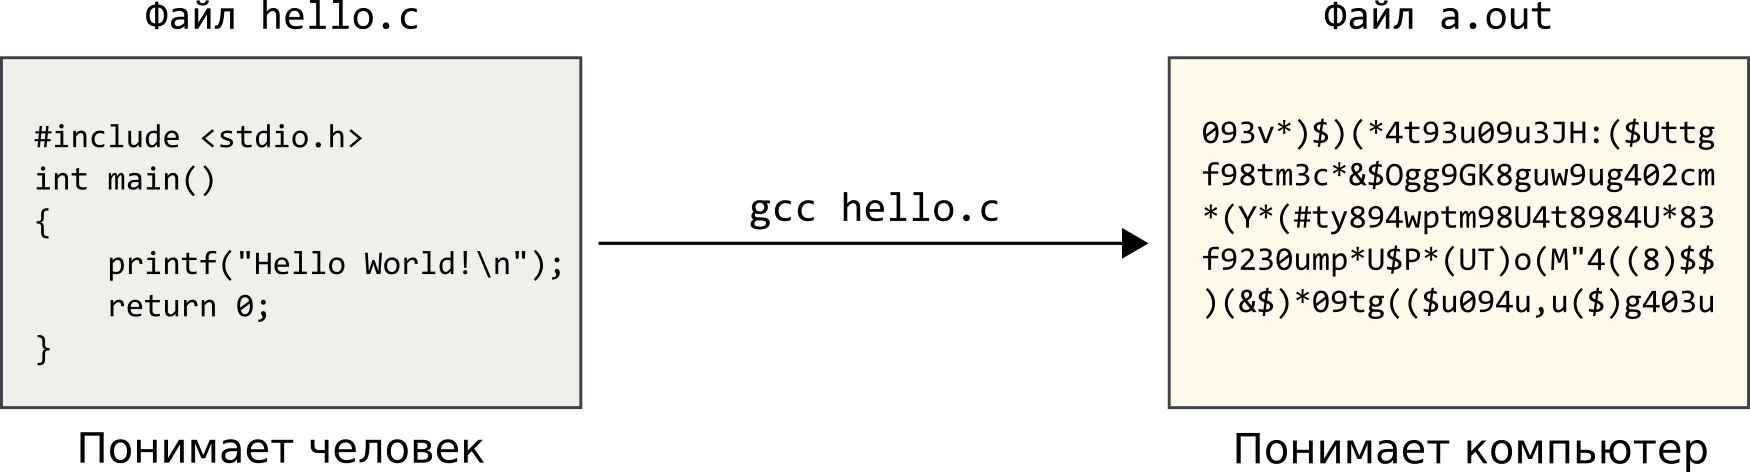
\includegraphics[scale=1]{../images/gcc_simple.png}
\end{center}

\subsection*{Горячие клавиши:}
\texttt{
\begin{tabular}{ c | c }
 Tab           & автозаполнение \\ 
 2 раза Tab    & показать возможные варианты \\ 
 стрелка вверх & перейти к предыдущей команде \\ 
 Ctrl-C        & выход из программы, например той, которая зависла в бесконечном цикле \\ 
 Ctrl-R        & поиск по всем предыдущим командам \\ 
\end{tabular}
}




\subsection*{Задание на работу с командной строкой:}
\begin{enumerate}
\item Откройте терминал и узнайте в какой папке вы находитесь. Для этого напечатайте \texttt{pwd} и нажмите \texttt{Enter}.
\item Перейдите в папку  \texttt{/home-local/student}. Для этого введите команду:
\begin{verbatim}
cd /home-local/student
\end{verbatim}
\item С помощью команды \texttt{pwd} проверьте, что вы действительно находитесь в нужной папке.
\item С помощью команды \texttt{ls} просмотрите всё содержимое папки \texttt{/home-local/student}. Для этого введите \texttt{ls} и нажмите \texttt{Enter}.
\item Создайте вашу папку, в которой вы будете работать в течении семестра. Используйте команду:
\begin{verbatim}
mkdir имя_папки
\end{verbatim}
За место \texttt{имя\_папки}  подставьте название вашей папки. Желательно, чтобы название содержало только латинские символы без пробелов.
\item С помощью команды \texttt{ls} убедитесь, что ваша папка создалась.
\item Перейдите в вашу созданную папку командой \texttt{cd имя\_папки}.

\item Перейдите в эту папку с помощью файлового менеджера(проводника) и создайте там файл \texttt{hello.c}. Файл обязан оканчиваться на \texttt{.c}.

\item С помощью обычного текстового редактора (например, gedit или Sublime Text) напишите в файле \texttt{hello.c} текст программы \textit{HelloWorld}:
\begin{lstlisting}
#include <stdio.h>
int main() 
{
    printf("Hello World\n");
}
\end{lstlisting}

\item В терминале проверьте, что этот файл существует, используя команду \texttt{ls}.
\item Скомпилируйте этот файл следующей командой:
\begin{verbatim}
gcc hello.c
\end{verbatim}
После этого в папке создастся новый файл по имени \texttt{a.out}.
\item Запустите исполняемый файл \texttt{a.out} напечатав полный путь до этого файла:
\begin{verbatim}
/home-local/student/ваша_папка/a.out
\end{verbatim}
\item Точка в имени файлового пути является сокращением для текущей папки. То есть в данном случае точка является сокращением для \texttt{/home-local/student/ваша\_папка}. Поэтому команду для запуска файла \texttt{a.out} можно сократить до:
\begin{verbatim}
./a.out
\end{verbatim}
\item Можно объединить команды компиляции и запуска:
\begin{verbatim}
gcc hello.c && ./a.out
\end{verbatim}
Измените программу так, чтобы она печатала \texttt{Hello MIPT!}, скомпилируйте и запустите программу. \\
\textit{Примечание}: каждый раз вводить эту команду не нужно, можно просто нажать клавишу вверх, чтобы исполнить предыдущие команды.


\item Перейдите в папку \texttt{code/1int}, используя \texttt{cd}.

\item Скомпилируйте и запустите программу \texttt{01print\_int.c} с помощью команды
\begin{verbatim}
gcc 01print_int.c && ./a.out
\end{verbatim}
Эта программа должна напечатать на экран:
\begin{verbatim}
My name is Alex
I am 10 years old
\end{verbatim}

\item Перейдите в папку \texttt{code/0hello}, используя \texttt{cd}:
\begin{verbatim}
cd ../0hello
\end{verbatim}

\item Скомпилируйте и запустите программу \texttt{00hello.c} с помощью команды
\begin{verbatim}
gcc 00hello.c && ./a.out
\end{verbatim}
Эта программа должна напечатать на экран \texttt{Hello World}.


\end{enumerate}

\end{document}